\section{The Representative Anonymization Algorithm}
\label{sec:repOB}
Instead of designing new methods for \emph{uncertain} graphs, we first consider somehow utilizes methods for deterministic graphs. Fortunately, there has been extensive work on extracting a single representative instance (deterministic one) of uncertain graphs that capturing graph statistics such as the expected vertex degrees~\cite{Parchas_Gullo_Papadias_Bonchi_2014}.  

Motivated by the preceding, in this work we introduce the representative anonymization (Rep-An) algorithm that combines isolated but complementary work from literature for uncertain graph anonymization. As shown in Figure\ref{fig:repOB}, we first extract a single \emph{representative} instance from an original uncertain graph. Then, conventional anonymization techniques can be then applied on this representative to attain closely approximate anonymized output of the original uncertain graph. This body of research comes to its aid that anonymization can be carried out on uncertain graphs, regardless of the uncertainty inherent in the data.


However, this approach has several limitations. First, the input edge uncertainties (probabilities) are no longer integrated into the anonymization process since they are detached from the graph in the first step. Second, the anonymization process (the second step) is oblivious to the {\em reliability} metric since its input is a made-up deterministic graph. Third, since the two phases are isolated from each other, different phases are optimized for different metrics. As the result, this naive \texttt{Rep-An} approach introduces a high level of noise and consequently deteriorates the overall utility of the anonymized graph. 
In the experiment section, we further study this approach empirically and confirm its impracticality.

\begin{figure}[t]
	\vspace{-1em}
    \captionsetup{margin=0cm}
    \centering  
        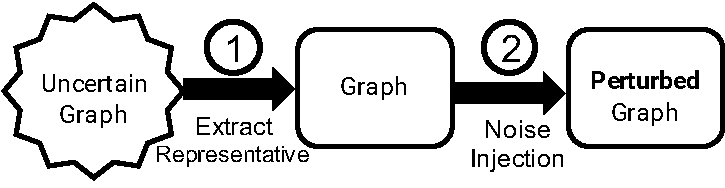
\includegraphics[width=0.95\columnwidth]{AddFigure/repOB.pdf}
        \vspace{-0.7em}
    	\caption{Overview of Rep-An. Noise is added to the extracted \emph{representative} instance.}
    \label{fig:repOB}
    \vspace{-0.5em}
\end{figure}
\subsection{Validation on Real Uncertain Graphs}
In this section, we empirically evaluate the impact of noise injected to extracted \emph{representative} instances by executing Rep-An on real uncertain graphs.

\textbf{Uncertain Graphs.}~~We use three uncertain graphs that capture different real-world scenarios and have been used in prior uncertain graph mining studies. Table~\ref{tab:dataset} lists uncertain graphs and their tolerance parameters used in our evaluation.

\textsc{DBLP} is a co-authorship network where the probability of an edge between two authors represents the likelihood two authors will collaborate in the future. The probability is obtained by a predictive model based on historical co-authorship data.~\cite{Jin_Distance_2011}. 

\textsc{Brightkite} is a location-based social network where the probability of an edge between two users corresponds to the chance that two users visit each other. The probability can be obtained by a prediction model based on historical data~\cite{Cho_Friendship_2011}.

\textsc{PPI} is a dataset of protein-protein interactions, provided by Disease Module Identification DREAM Challenge, where the probability of any edge corresponds to the confidence that the interaction actually exists.
The probability is obtained through biological experiments.

% Add one sentence 
\begin{table}[t]
    \centering
        \caption{Characteristics of the datasets and privacy parameters}
        \begin{tabular}{|c|c|c|c||c|}
        \hline 
        Graph    & Nodes    & Edges    &Edge Prob    & Tolerance level\\
        \hline  
        DBLP     &824,774   &5,566,096 & 0.46        & $10^{-4}$\\
        \small{BRIGHTKITE} &58,228   & 214,078 &0.29 &$10^{-3}$ \\
        PPI      &12,420   & 397,309  & 0.29         &$10^{-2}$\\
        \hline
        \end{tabular}
        \label{tab:dataset}
\end{table}

\begin{figure}[!htb]
  \subfigure[\small Edge Probability Distribution]{\label{subfig:edgepro}  
    \begin{minipage}[l]{1\columnwidth}
      \centering
       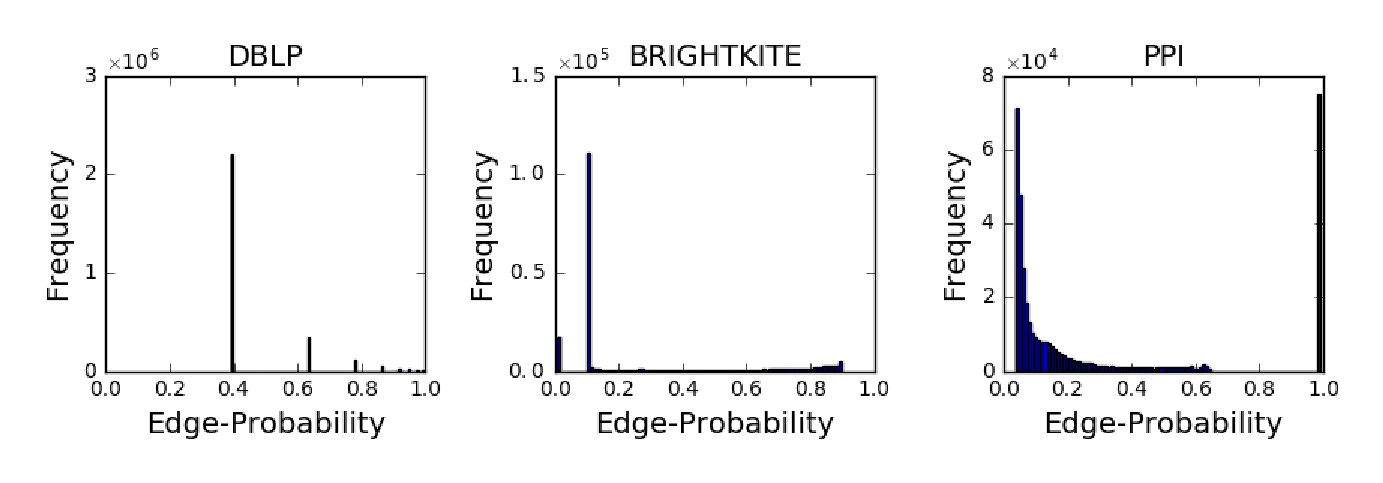
\includegraphics[width=\linewidth]{exp/edge_prob_row.eps}
    \end{minipage}
    \vspace{-15pt}
  }
  \subfigure[\small Expected Degree Distribution]{\label{subfig:degreepro}  
    \begin{minipage}[l]{1\columnwidth}
      \centering
       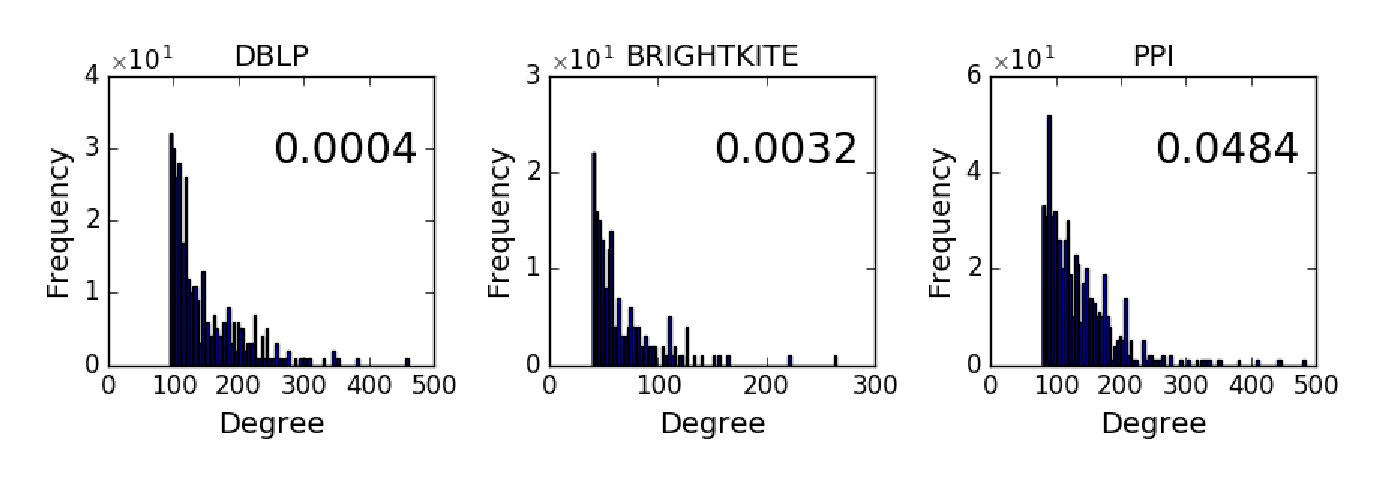
\includegraphics[width=\linewidth]{exp/degree_row.eps}
    \end{minipage}
  }
    \vspace{-10pt}
    \caption{Edge probability\& degree distributions.}
    \label{fig:summary_graph}
   \vspace{-15pt}
\end{figure}

Figure~\ref{subfig:edgepro} shows the edge-probability distribution in the three datasets. 
Note that the DBLP dataset only has  a few probability values, while Brightkite dataset's probability values are generally very small.The PPI dataset has a more uniform probability distribution. 
We also present their degree distributions of ``unique'' nodes (with high degree and obfuscation level is smaller than $300$). Observe that, all the three graphs have a heavy-tailed degree distribution (i.e, an amount of ``unique" nodes). In the context of graph privacy, the larger amount of ``unique'' nodes requires a larger amount of noise.


% pass 
\textbf{Computation.}~~We extract the single representative instances for each uncertain graph, introduce noise using the state-of-art graph anonymization strategy, and then compute the Reliability Discrepancy between the perturbed graph and the original uncertain graph as a measure of the level of graph structural error introduced. We approximate its expectation value by the average value obtained over the sampled possible worlds. Here, we use 1,000 samples since it has been shown that $1000$ usually suffices to achieve accuracy converge~\cite{Potamias_K_2010}.

\textbf{Results.}~~Figure~\ref{} shows that the Rep-An algorithm produces a large error for large values of $k$ (i.e. strong privacy guarntees). As we mentioned, the low level of utility is due to the large noise Rep-An injects into the representative instance, resulting in a perturbed graph (uncertain one) which is significantly different from the original \emph{uncertain} graph. 

The high discrepancy is largely due to the representative extraction step. In the extreme case where $k=1$ (i.e. no privacy guarntees), the sole representative extraction step produces high reliability errors. 
To better understand its limitation, we report the potential lower-bound on the error that could be achieved via Chamelon methods in Figure~\ref{}. Indeed, Figure~\ref{} shows that the utility loss of the Rep-An strategy can largely be attributed to the overlook of edge uncertainty.   
% add one sentence about the
% add more sentences to highlight their difference. 




